\chapter{Background}


%%%%%%%%%%%%%%%%%%%%%%%%%%%%%%%%
%         Cosmic-ray
%%%%%%%%%%%%%%%%%%%%%%%%%%%%%%%%
\section{Cosmic ray}
This section discusses the historical discoveries from early
studies in the field to the latest high-impact experiments. 

\subsection{History}
In 1909, Theodor Wolf conducted the famous experiment that
pioneered the study of cosmic rays (CRs) by taking an apparatus
to measure the rate of ionization from the ground to the top of
the Eiffel Tower in Paris \citep{gray1949cosmic}.
% the famous experiment that pioneer the study of CR has been
% led by Theodor Wolf who takes conduct the experiment of 
% altitude variation by taking the apparatus to measure 
% the rate of ionization from the ground to the top of 
% the Eiffel Tower in Paris \citep{gray1949cosmic}.
The result showed that the ionization rate was increased
but the magnitude is much lower than the expectation from 
the underground radioactivity which provided a clue
that the origin of CRs was from outer space
rather than from the Earth \citep{EarlyCRGerman}.

\begin{figure}[h!]
    \centering
        \subfloat[
            An early version schematic view of
            electrometer used by Thedor Wulf
        ]{
            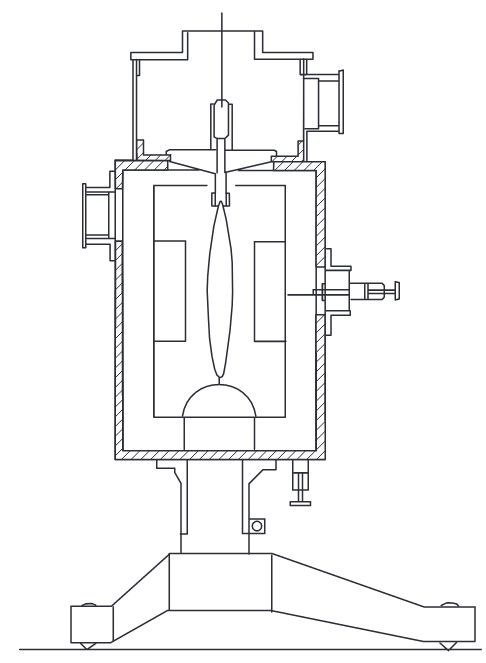
\includegraphics[width=0.32\textwidth]{content/background/figures/wulf_schema.png}
            }
        \hfill
         \subfloat[
            Ionization rate from Victor Hess (left) and Werner
            Kolhörster (right)
         ]{
            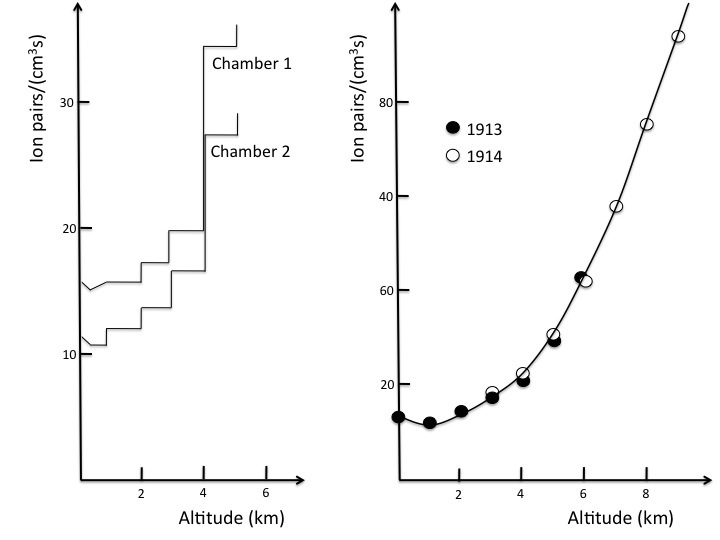
\includegraphics[width=0.6\textwidth]{content/background/figures/HessKol.jpg}
            }
        \caption{Wulf's apparatus and the balloon experimental results}
       \label{fig:xxx}
\end{figure}


However, the experiment measuring the effect of altitude
variation with a tiny altitude scale compared to the Earth's
atmospheric thickness may not provide enough data.
% atmosphere would not enough to consolidate the theory.
% In the same year, the ballon with a similar instrument has
% been released up to 1.3 kilometers by Karl Bergwitz to put more
% weight on the first experiment.
They found that the ionization rate
has increased by a quarter compared to that at ground level
\citep{de2014atmospheric}.
Three years later, a risky investigation was conducted by 
an Australian gentleman who brought a detector and himself
to fly with a balloon.
His name is Victor Hess, and his name went so famous
because he risked his life with the experiment 
and his flying over 5 kilometers above the ground \citep{hess1912beobachtungen}.
The result is strongly significant and impactful
to the astrophysical research community. Risking life  
In 1914, Werner Kolhörster repeated the balloon experiment 
with higher altitude up to 9 kilometers from 
sea level and the ionization rate still increased when 
the ballon flew higher. These results emphasized that the source of 
the ionizing ray came from Earth's upper atmosphere
or the outer space.

% Main  points  where  CR  intensities  were  measured  during  eight Compton expeditions in 1932 

\begin{figure}[h!]
    \centering
        \subfloat
        {
            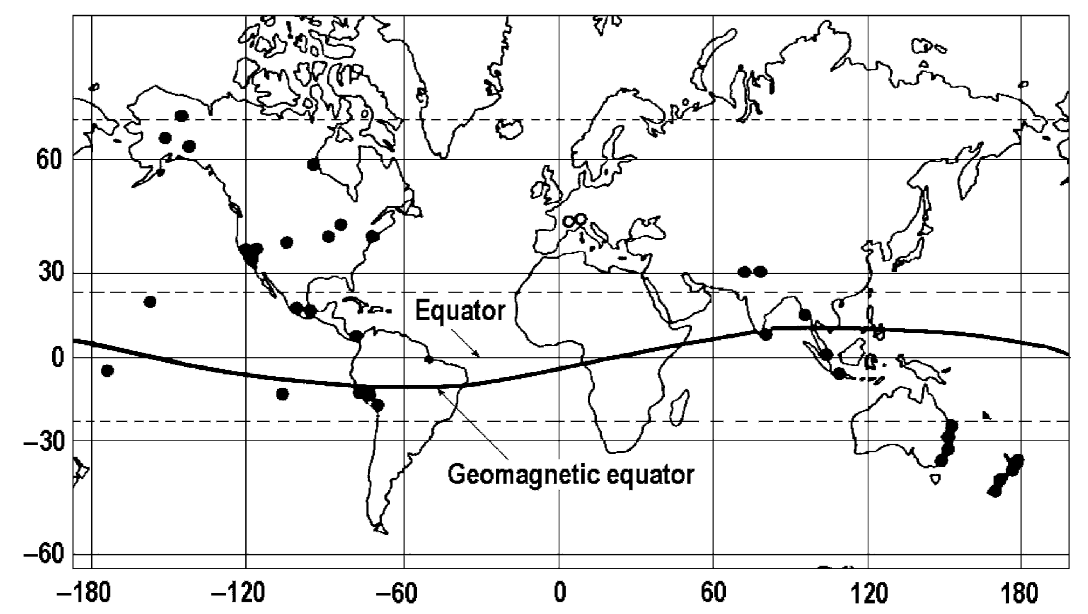
\includegraphics[width=0.62\textwidth]{content/background/figures/clay_geographical.png}
        }
        \hfill
        \subfloat
        % [
        %     The Pb-shielded ionization chamber, 
        %     organized by Compton. Image taken from
        %     \cite{text_cr_geomagnetic_effect}   
        % ]
        {
            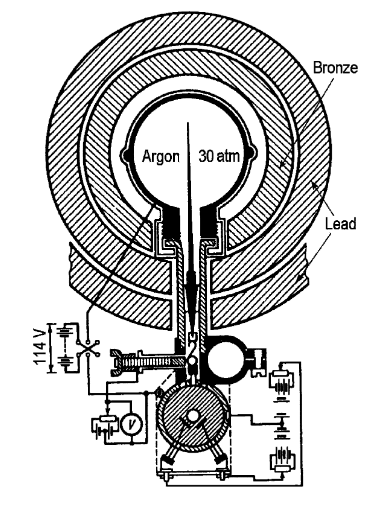
\includegraphics[width=0.32\textwidth]{content/background/figures/compton_pb_shield.png}
        }
        \caption{
            (left) Clay's experiment on the geographical variation
            of CR intensity. Main locations where CR intensity was
            measured during 8 Compton's expeditions in 1932.
            (right) The Pb-shielded ionization chamber, 
            organized by Compton. Image is taken from
            \cite{text_cr_geomagnetic_effect} 
        }
       \label{fig:clay_cr_ship}
\end{figure}

% Not only the altitude variable that related to the 
% the intensity of the CRs, but the geographic location of the 
% observation also does affect the measurement.
Not only does the ionization rate varies with altitude,
the measured rate also depends on the geographical locations.
The first experiment was done by John Clay who
sailed the ship across the ocean from Holland to Java
\citep{Clay1927,Clay1928}. The geographical locations
% that are used to measure the CR intensities
where CR intensities were measured
and the apparatus schematical draft are shown in Figure
\ref{fig:clay_cr_ship}. The result shows that
the further from the equator, the higher CR intensity.
Another exploration for the geographic variation was 
done by John Compton in the following five years.
He sailed the ship from Sydney (southern hemisphere)
to Vancouver (northern hemisphere) for various seasons
from 1936 to 1937 back and forth \citep{compton1937cosmic}.
Figure \ref{fig:comptonship} demonstrates the 
latitude variation and the seasonality effects of the 
multiple trips from the experiment.

\begin{figure}[h!]
    \centering
    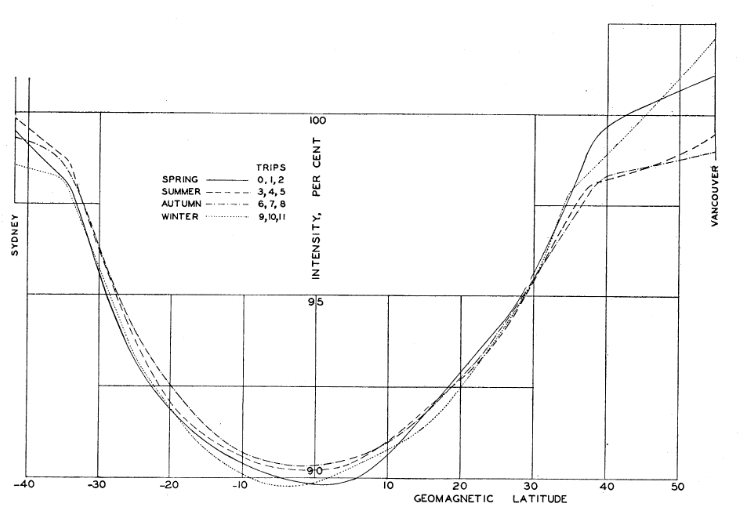
\includegraphics[width=\textwidth]{content/background/figures/compton_sail_1937.png}
    \caption{
        Latitude variation of CR intensity for various seasons 
        % Latitude variation for various seasons
        \citep{compton1937cosmic}
    }
    \label{fig:comptonship}
\end{figure}
	
The first interpretation study from the discovery has been
done by \cite{stormer1934critical}. The explanation of the CR's altitude variation
came from the trajectory of CR particles due to geomagnetic field.
In that period, the topic of the geomagnetic field
effects on CRs were quite famous.
Another impactful study of the
CR trajectories under the influence of the
Earth's magnetic field was conducted by
Bruno Rossi. He studied an assymetry of the East-West distribution
of CR flux due to the Lorentz force effects on charged particles
by the Earth's magnetic field. He found that the flux is enhanced
from the West and interpreted that CRs are predominantly
positively charged \citep{rossi1941cosmic}.
% Bruno Rossi
% for predicting an asymmetry of the East-West distribution
% of CR spectrum because the primary CRs does have a positive or
% the negative charge than the cyclic moving direction of the 
% the particle was induced by Lorentz force where the direction of 
% the Earth's magnetic field could be identified to determine the
% direction of the charged particles \citep{rossi1941cosmic}.


% A ground-based detector is a great option for 
% detecting the CRs where it includes primary and secondary CRs.
% However, investigating the primary CRs is a challenging topic
% for ground-based detectors especially for low energy particles.
% Another interesting option to inspect the asymmetry of 
% East-West could be done by using a space-based detector 
% that orbit around the Earth's at some radius in the
% the higher altitude and it would face a lower 
% the atmospheric density which considers to be an interesting 
% the choice to study the CRs with a lower effect of atmospheric
% interaction. In 2008, \textit{Fermi} Large Area Telescope (LAT)
% has been launched to observed $\gamma$-ray and
% lightweight lepton particles which are electron
% and position. The East-West effects from geomagnetic
% induction was also emphasized by \textit{Fermi}-LAT.


\subsection{Physical properties}
CRs are high-energy particles propagating through
space. CRs gain their momentum from
various acceleration mechanisms CRs gain their momentum
such as supernovae, created by astrophysical objects.
The composition of CRs consists of approximately
90\% protons, 8\% alphas, and other nuclei of heavier
elements \citep{CRComposition2017}. Experimentally,
many observations indicate that the CR spectra for all particles
and individually do follow the power law in rigidity
(momentum per charge)
for which the spectral index depends on the
energy range. Theoretically, the observed spectrum
in a broad energy range
is the superposition of CRs produced by various types of
sources which could exhibit different spectral indices
depending on their physical properties.



\begin{figure}[h!]
    \centering
    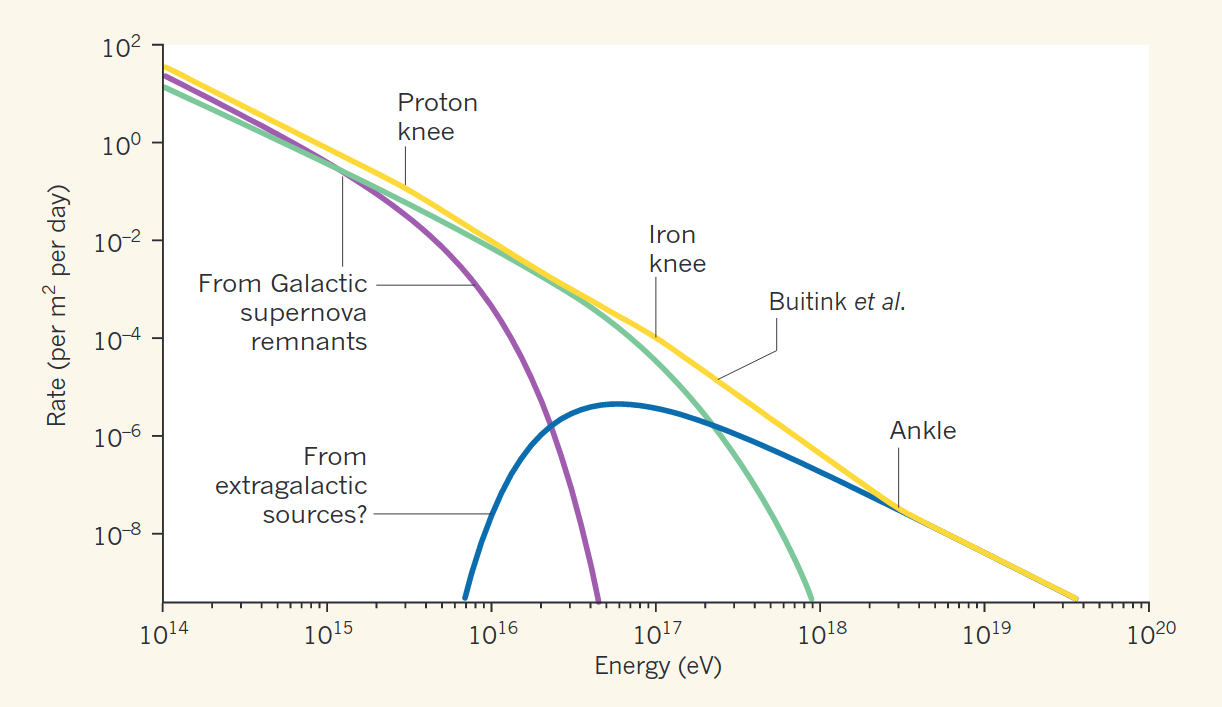
\includegraphics[width=\textwidth]{content/background/figures/andrew_superposition.png}
    \caption{
        The CR spectrum showing the superposition of different
        populations of sources
        \citep{taylor2016_crspectrumsuperposition}
    }
    \label{fig:cr_superposition}
\end{figure}

% As mentioned in an early paragraph, each source of CR does reflect their
% own specific spectral index in the arrival CR spectrum.
% To validate the theoretical assumption, putting the simulation or calculation of each source and check
% with the real data does compliment experimental observations.
% The superposition of various sources that yield a 
% discontinuity of the spectral indices has been exploited
% in some energy ranges.
% Two well-known breaking points 
% are knee and ankle where it located in the energy order around $10^{15}$ eV and $10^{18}$ eV sequentially.
Figure \ref{fig:cr_superposition} shows the widely accepted
scenario of how each population of CR sources dominates the
value of the spectral index for different energy ranges.
Three well-established spectral breaking points are the first knee
at $\sim10^{15}$ eV, the second knee at $\sim10^{17}$ eV,
and the ankle at $\sim10^{19}$ eV.
The rate to find one particle with the energy above the first knee
is around one particle per square meter per year and 
the possibility that an apparatus could detect
% the particle in energy at ankle point is
a particle at energy above the ankle is roughly one particle per 
kilometer per year.
% Figure \ref{fig:cr_superposition} illustrate
% the concept of superposition from various sources and 
% yield the arrival CR spectrum with breaking spectral indices. 


% Not only the below ankle energy that has an interesting property, but the CR that has energy beyond the ankle energy
% also has an identical property. It knowns as ``ultra-high
% energy cosmic rays'' (UHECR). One interesting point is that
% it does not that far from the ankle in terms of rigidity magnitude
% which higher around 1 or 2 order of magnitude.
Interestingly, the maximum energy of UHECRs ever detected never
exceed $\sim$2 orders of magnitude above the ankle energy.
% The widely known 
% explanation why it could not go so far is the
This upper energy limit of CRs is widely known as the
Greisen–Zatsepin–Kuzmin (GZK limit).
According to the GZK theory, UHECRs cannot have an energy above
a certain limit because UHECRs are produced from distant
extragalactic sources and propagate through vast space full
of low-energy background photons, the cosmic microwave background. 
According to the GZK theory, UHECRs cannot have an energy above
a certain limit because UHECRs are produced from distant
extragalactic sources and propagate through vast space full
of low-energy background photons, the cosmic microwave background. 
When the energy of the UHECRs is above a certain threshold,
they would interact with the background photons and lose their
energies \citep{gzk_cr_limit}. 


% The theory provides the description of why the UHECR
% could not propagate though the space but please note that
% some sources still could produce such a UHECR but the main
% the issue here it the space does not empty. It contains some 
% intermediate matter or dust and the microwave background radiation
% which it is believed that came from the residue of the 
% Big Bang or some great explosion or expansion of the space that 
% human never saw it (at least in the human lifetime).
% The main calculation of the CR kinetic energy limit from GZK 
% was considered only proton particles and the main interaction
% that makes it stop is basically from the interaction with 
% microwave background radiation that almost perfectly
% isotropically propagating in the space with an order of 
% traveling proton around hundred light-years in the space
% \citep{gzk_cr_limit}. The way of this kind of interaction 
% not only does slow down the CR proton by producing 
% neutral pion where it mostly decays into a pair of $\gamma$-rays
% but it could also yield a neutron with 
% a charged pion. Hence, it also answers why we could 
% see such a high energy neutron that does not only 
% produced in the sky (shower effects) albeit it does not
% has any charge to be accelerated in the famous 
% acceleration mechanism such as shock acceleration.


CRs can be categorized into two types based on
how they are produced:
\begin{enumerate}
    \item \textbf{Primary cosmic rays}:
    are produced from astrophysical objects which may be within the
    Solar system, within the Milky Way Galaxy (Galactic CRs), or
    from extragalactic sources (extragalactic CRs). Some example
    origins of primary CRs are stellar winds, supernovae, pulsars,
    active galactic nuclei, and speculative sources such as dark
    matter decay.
    % they mostly are produced from the
    % Solar system, somewhere in the Milky ways, extragalactic sources and many more. When they interact with the Earth's atmosphere,
    % with the hadronic interaction with the air molecules,
    % they produce the secondary CR particles.
    \item \textbf{Secondary cosmic rays}:
    are produced from primary CRs interacting with the Earth's
    atmosphere. The interactions create showers of hadronic,
    leptonic, and electromagnetic particles. Researchers have
    developed and improved Monte Carlo simulations of the
    CR air showers based on particle physics theory. These models
    are very useful for secondary CRs studies.
    % as mentioned in collapsing of the  
    % primary CRs, secondary CRs consists of many particles
    % from lightweight leptons to medium weight leptons and 
    % from mesons to hadron particles as well. The interaction
    % of the proton with the atmospheric molecule looks simple 
    % but the precise calculation from derivation is extremely complicated 
    % since there is the endless possibility of the (Feynman) path that 
    % also produce other products with a certain probability.
    % By the end of the day, we got a few certain 
    % of particles from their likelihood of the occurrence from 
    % the collision which mainly are electrons, positions, muons,
    % pions and photons as demonstrates in Figure \ref{fig:cr_shower}.
\end{enumerate}

\begin{figure}[h!]
    \centering
    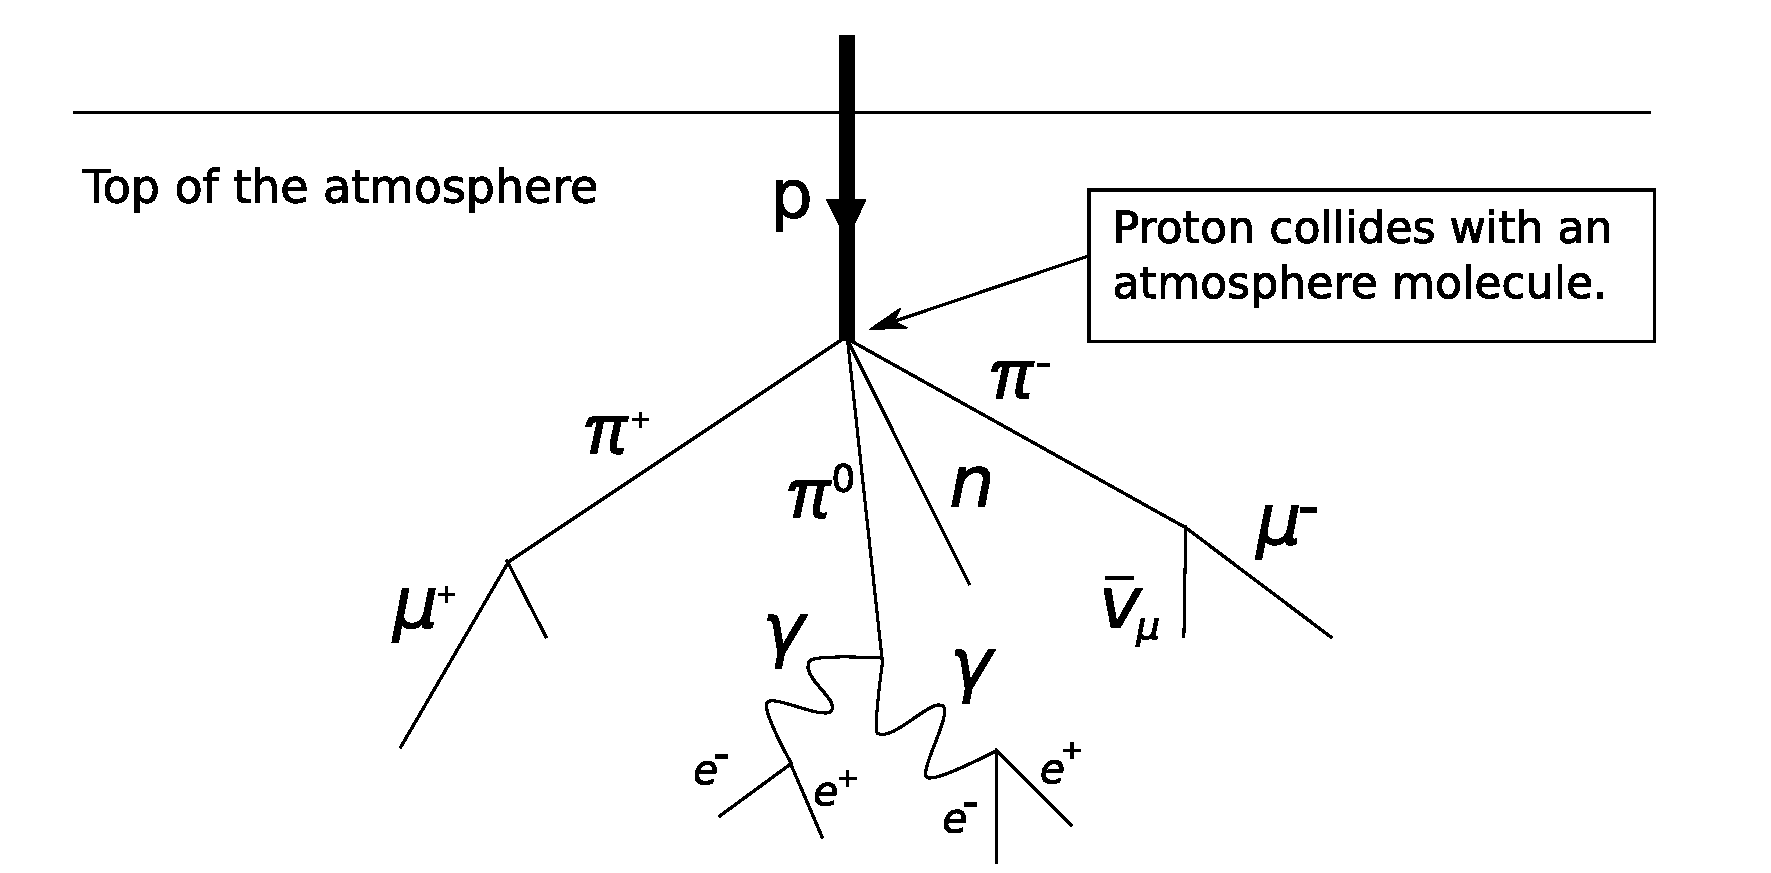
\includegraphics[width=\textwidth]{content/background/figures/Atmospheric_Collision.pdf}
    \caption{
        % Cosmic rays shower from collision of primary CR with the atmospheric molecule
        Simplified schematic of CR proton air shower
        (Image taken from Cosmic Rays, Wikipedia, Magnus Manske, 2011)
    }
    % 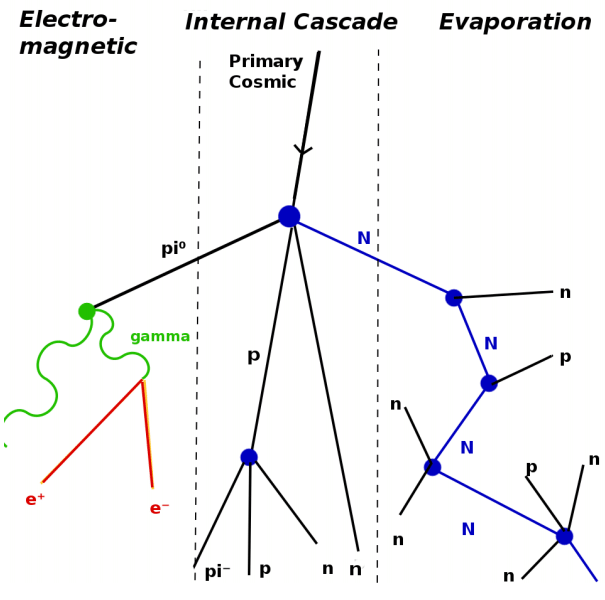
\includegraphics[width=0.7\textwidth]{content/background/figures/cr_shower2.png}
    % \caption{Cosmic rays shower from collision of primary CR with the atmospheric molecule.
    % Image taken from \cite{cr_shower_img}
    % }
    \label{fig:cr_shower}
\end{figure}


\subsection{$\gamma$-ray production}

The production mechanisms of $\gamma$ rays are fundamentally
different from those for charged particles that can be
accelerated with the electromagnetic force.
While charged particles can gain or lose energy during their
propagation through space, high-energy $\gamma$-ray photons
tend to only lose energy.
Here we briefly discuss the production processes of $\gamma$ rays.
% The production of $\gamma$-ray particles happens all the 
% time. It is mandatory to understand how a photon could 
% gain a very high momentum from nature. The procedure 
% to acquire all those kinetic energies is quite different from how
% a charged particle obtains its momentum because a 
% the charged particle could earn their kinetic energy during 
%  their trip of propagating through space with a 
% Lorentzian force. The $\gamma$-rays mostly have only one 
% chance to pick their kinetic energy and it happens when it 
% was produced because it is barely interact with any other 
% particles in the space especially high energy $\gamma$-ray.
% The scenarios that make photon hold high energy are 
% listed in the following bullets.

% \subsubsection{Mechanism of $\gamma$-ray producing}

\begin{itemize}
    \item \textbf{Decaying of unstable matter}:
    Radioactive decay is one of the most well-known phenomena for the $\gamma$-decay mode. One example of heavy-ion decay is cobalt-60. It decays 
    into an excited state of nickel as

    \ch{27^{60}Co -> 28^{60}Ni^{*} + e- + $\bar{\nu}$ + $\gamma$},

    then the excited nickel
    emits another $\gamma$ ray to become the stable state
    % decay another $\gamma$-ray
    % to make it to the stable state

    \ch{28^{60}Ni^{*} -> 28^{60}Ni + $\gamma$ }.

    Some particles, such as the neutral pion ($\pi^0$),
    decay into $\gamma$ rays.
    The Feynman's diagram of a $\pi^0$ decay is demonstrated in
    Figure \ref{fig:neutral_pion_decay}.
    The lifetime of $\pi^0$ is short, $\sim 8.5\times10^{-17}$ seconds.
    % The famous decay of a lower level from a small nucleus that consists of two quarks called "meson".
    % To be more precise, it is known as the pion decay.    
    % The path diagram is demonstrated in Figure \ref{fig:neutral_pion_decay}
    % where the neutral pion from the collision process that interacts
    % via Yukuwa's interaction. The neutral pion itself does not stable
    % then it would have a short amount of lifetime before it mostly
    % decays into two high-energy photons.
    \begin{figure}[h!]
        \centering
        \begin{tikzpicture}
    \begin{feynman}
    \vertex (a);
    \vertex [below= of a] (b);
    \vertex [left= of a] (p1) {\(u\)};
    \vertex [left= of b] (p2) {\(\bar{u}\)};
    \vertex [right= of a] (q1) {\(\gamma\)};
    \vertex [right= of b] (q2) {\(\gamma\)};
    
        \diagram* {
            (p1) -- [fermion] (a) ,
            (a) -- [fermion] (b),
            (b) -- [fermion] (p2) ,
            (a) -- [photon] (q1),
            (b) -- [photon] (q2),
        };
    \end{feynman}
\end{tikzpicture}
% \begin{tikzpicture}
%     \begin{feynman}
%     \vertex (a);
%     \vertex [below= of a] (b);
%     \vertex [left= of a] (p1) {\(d\)};
%     \vertex [left= of b] (p2) {\(\bar{d}\)};
%     \vertex [right= of a] (q1) {\(\gamma\)};
%     \vertex [right= of b] (q2) {\(\gamma\)};
    
%         \diagram* {
%             (p1) -- [fermion] (a) ,
%             (a) -- [fermion] (b),
%             (b) -- [fermion] (p2) ,
%             (a) -- [photon] (q1),
%             (b) -- [photon] (q2),
%         };
%     \end{feynman}
% \end{tikzpicture}

% \begin{tikzpicture}
%     \begin{feynman}
%         \vertex (a);
%         \vertex [above right= of a] (b);
%         \vertex [below right= of a] (c);
%         \vertex [left= of a] (p1) {\(\pi^0\)};
%         \vertex [right= of b] (q1) {\(\gamma\)};
%         \vertex [right= of c] (q2) {\(\gamma\)};

%         \diagram* {
%             (p1) [particle] -- [scalar] (a),
%             (a) -- (b),
%             (a) -- (c),
%             (b) -- (c),
%             (b) -- [photon] (q1),
%             (c) -- [photon] (q2),
%         };
%     \end{feynman}
% \end{tikzpicture}
        \caption{Feynman's diagram of the neutral pion ($\pi^0$) decay into two $\gamma$-rays.}
        \label{fig:neutral_pion_decay}
    \end{figure}
    There are some other decay channels (with $<1$\% branching
    ratio) that result in combinations of a photon and pairs of
    lightweight leptons, as long as the momentum, energy, and
    quantum numbers are conserved.
    % Neutral pion also could yield one $\gamma$-ray
    % and a pair of lightweight leptons, a couple 
    % pair of lightweight leptons or even just a pair 
    % of lightweight leptons and much more as long as it 
    % conserve the momentum, energy and quantum numbers.
    % The main reason why the majority of their decaying process
    % does yield only photons because the scattering amplitude
    % as the Figure \ref{fig:neutral_pion_decay} does hold a branching
    % ratio around 0.98823 and the rest of them are 
    % smaller than 1\%.
    Another interesting property of the $\pi^0\rightarrow 2\gamma$ mode
    is the momentum
    vectors of the $\gamma$-ray pair have the same magnitude but
    opposite direction in the rest frame of $\pi^0$.
    % vector of their pair $\gamma$-ray
    % hold an opposite direction with the same amplitude in the 
    % reference frame.

    \item \textbf{electron–positron annihilation}:
    Electron ($e^-$) and positron ($e^+$) are the lightest
    leptons which can annihilate into 2 $\gamma$-rays.
    Heavier and shorter-lived leptons, muon ($\mu$) and
    tau ($\tau$), can also create $\gamma$ rays in a similar
    manner as illustrated in Figure \ref{fig:lepton_annihilation}.
    % In the universe, there is some probability of the electron and position was forced to face each other by some chance from the electromagnetic force or randomly found each other.
    % The interaction when they facing each other dominate by electromagnetic interaction and requires a photon as a mediator to allow them to talk to each other from a quantum electrodynamics point of view. There is a change 
    % when those pair of leptons decide to annihilate into high energy photons
    % without running any physical laws. Nevertheless, another kind of
    % a pair of leptons like muon technically could deform into two
    % photons with much higher energy because their rest mass is higher.
    % Surely, a pair of Tau is also allowed to produces a pair of photons.
    % However, the lifetime of those medium-weight and heavy-weight leptons could not last that long to survive in practical. The simplest 
    % Feynman's path of annihilation of leptons into a pair of photons 
    % is illustrated in Figure \ref{fig:lepton_annihilation} from light 
    % to heavy leptons sequentially.

    \begin{figure}[h!]
        \centering
            \subfloat[
                Lightweight leptons
            ]{
                \begin{tikzpicture}
\begin{feynman}
\vertex (a);
\vertex [below= of a] (b);
\vertex [above left= of a] (p1) {\(e^{-}\)};
\vertex [below left= of b] (p2) {\(e^{+}\)};
\vertex [above right= of a] (q1) {\(\gamma_1\)};
\vertex [below right= of b] (q2) {\(\gamma_2\)};

    \diagram* {
        (p1) -- [fermion] (a) ,
        (a) -- [fermion] (b),
        (b) -- [fermion] (p2) ,
        (a) -- [photon] (q1),
        (b) -- [photon] (q2),
    };
\end{feynman}
\end{tikzpicture}
            }
            \hfill
            \subfloat[Mediumweight leptons]{
                \begin{tikzpicture}
    \begin{feynman}
    \vertex (a);
    \vertex [below= of a] (b);
    \vertex [above left= of a] (p1) {\(\mu^{-}\)};
    \vertex [below left= of b] (p2) {\(\mu^{+}\)};
    \vertex [above right= of a] (q1) {\(\gamma_1\)};
    \vertex [below right= of b] (q2) {\(\gamma_2\)};
    
        \diagram* {
            (p1) -- [fermion] (a) ,
            (a) -- [fermion] (b),
            (b) -- [fermion] (p2) ,
            (a) -- [photon] (q1),
            (b) -- [photon] (q2),
        };
    \end{feynman}
    \end{tikzpicture}
            }
            \hfill
            \subfloat[
                Heavyweight leptons
             ]{
                \begin{tikzpicture}
    \begin{feynman}
    \vertex (a);
    \vertex [below= of a] (b);
    \vertex [above left= of a] (p1) {\(\tau^{-}\)};
    \vertex [below left= of b] (p2) {\(\tau^{+}\)};
    \vertex [above right= of a] (q1) {\(\gamma_1\)};
    \vertex [below right= of b] (q2) {\(\gamma_2\)};
    
        \diagram* {
            (p1) -- [fermion] (a) ,
            (a) -- [fermion] (b),
            (b) -- [fermion] (p2) ,
            (a) -- [photon] (q1),
            (b) -- [photon] (q2),
        };
    \end{feynman}
    \end{tikzpicture}
            }
            \caption{Lepton-antilepton annihilation path diagram.}
           \label{fig:lepton_annihilation}
    \end{figure}

    \item \textbf{Synchrotron \& Bremsstrahlung radiation}:
    It is theoretically and experimentally well known that when
    charged particles are accelerated, they emit photons.
    If the acceleration is due to a magnetic field, the emission
    is called the synchrotron radiation. Humans have built
    donut-shaped apparatuses inside which charged particles
    are traveling in a circle guided by strong magnetic fields
    and produce synchrotron radiation for various applications.

    Another closely related mechanism is the Bremsstrahlung process.
    When charged particles, typically electrons, move close to
    heavier positively charged nuclei, the Coulomb force between
    them cause an acceleration on the electrons, resulting in
    Bremsstrahlung radiation.
    % The phenomena of turning the momentum direction of charged particles or accelerate into another direction share a similar description. Conservation of momentum has come into place when considering the bending charged particle that would emit the photon. Regarding the incoming direction of a charged particle and then turning it direction by $\pi/2$ radians. The question
    % that comes into mild is where does those initial momentum in an 
    % the incoming direction does since the momentum is conserved along 
    % the cartesian direction, not only the magnitude. Now the clue is 
    % here, they have to emit the photon to converse the momentum of 
    % the system.
    
    % Let walk through the first example called synchrotron radiation.
    % Keeping some charged particle circulating the donut-like
    % apparatus have some cost to pay to make them stay without
    % escaping the tunnel. Unquestionably, dragging some moving
    % particle circulating at some point requires a
    % centripetal force. In this case, applying electromagnetic
    % force without touching it would yield a radiation called
    % synchrotron emission.

    % The second mechanism is Bremsstrahlung, where a charged particle 
    % or typically an electron moving path close to some opposite charged 
    % particle or typically a proton. The explanation from Coulomb's law
    % would cover this scheme for the definition that the force is 
    % inverse proportional to the distance between two charges. Then 
    % moving past by an oppositely charged particle does induce the electron
    % bending and emit the photon because the explained reason from the 
    % previous paragraph. This mechanism happens when CR electrons 
    % moving through the matter of the Sun's chromosphere and interact with 
    % a positive charged and produce some high energy photon but usually 
    % it produces in the X-ray energy range.


\end{itemize}



% decel & ac cel
% \subsubsection{Mechanism of $\gamma$-ray gaining momentum}

% Even though, $\gamma$-ray usually does not prefer
% to talk to other fundamental particles because
% scattering amplitude of their interaction is pretty 
% low. Nonetheless, there are some scenarios that $\gamma$ could 
% gain more kinetic energy and losing their kinetic energy 
% when they traveling in the universe.

\begin{itemize}
    \item \textbf{Inverse Compton scattering}
    
    scattering: A photon can electromagnetically interact with an
    electron (or any charged particles). The Compton scattering
    describes a photon losing its energy to an electron.
    In the opposite situation, a highly relativistic electron
    can interact and transfer its energy to a low-energy photon
    to become a $\gamma$-ray photon. This process is called the
    ``Inverse Compton scattering'' as shown in Feynman's
    diagram in Figure \ref{fig:compton_feynman}.
    % The scattering of a photon (massless particle) with an electron 
    % (massive particle) could occur during their trip. Equation \ref{eq:inv_compton} 
    % demonstrate the symbolic relation of the scattering with the 
    % electromagnetic interaction and yield the same particles as an 
    % incoming particles.

    % \begin{equation}
    %     e^-\gamma \rightarrow e^-\gamma
    %     \label{eq:inv_compton}
    % \end{equation}

    % Interaction between an electron and a photon could make them converting the momentum via the scattering process. Since the system momentum has to be conserved,
    % then there will be one losing momentum and another one gaining momentum or kinetic energy. Suppose one photon is traveling and hits an electron or a charged particle, it could transfer the kinetic energy to the particle and their wavelength will be longer. In another word, it is losing kinetic energy.
    % On the other hand, this scenario could happen oppositely.
    % There is a situation when a high energy electron interacting with the photon and turns over its kinetic energy to the photon. After that,
    % a photon could gain more kinetic energy during their trip. 
    % The latter scenario is called "Inverse Compton Scattering".
    % The most likelihood choice of the interaction of the scheme
    % could be represented in Feynman's path as in
    % Figure \ref{fig:compton_feynman}.

    \begin{figure}[h!]
        \centering
            \subfloat[First branch]{
                \begin{tikzpicture}
    \begin{feynman}
    \vertex (a);
    \vertex [right= of a] (b);
    \vertex [below left= of a] (p1) {\(e^{-}\)};
    \vertex [above left= of a] (q1) {\(\gamma_1\)};
    \vertex [below right= of b] (p2) {\(e^{-}\)};
    \vertex [above right= of b] (q2) {\(\gamma_2\)};
  
      \diagram* {
        (a) -- [fermion, edge label'=\(\)] (b) ,
        (q1) -- [photon, momentum] (a) ,
        (p1) -- [fermion] (a),
        (b) -- [photon, momentum] (q2),
        (b) -- [fermion] (p2),
      };
      \vertex [below= 0.5em of a] {\(\)};
      \vertex [below= 0.5em of b] {\(\)};
    \end{feynman}
  \end{tikzpicture}
                }
            \hfill
             \subfloat[
                Second branch
             ]{
                \begin{tikzpicture}
    \begin{feynman}
    \vertex (a);
    \vertex [right= of a] (b);
    \vertex [below left= of a] (p1) {\(e^{-}\)};
    \vertex [above left= of a] (q1) {\(\gamma_1\)};
    \vertex [below right= of b] (p2) {\(e^{-}\)};
    \vertex [above right= of b] (q2) {\(\gamma_2\)};
  
      \diagram* {
        (a) -- [fermion, edge label'=\(\)] (b) ,
        (q1) -- [photon, momentum] (b) ,
        (p1) -- [fermion] (a),
        (a) -- [photon, momentum] (q2),
        (b) -- [fermion] (p2),
      };
      \vertex [below= 0.5em of a] {\(\)};
      \vertex [below= 0.5em of b] {\(\)};
    \end{feynman}
  \end{tikzpicture}

                }
            \caption{
                % Trivial Feynman's path of (Inverse) Compton scattering
                First-order Feynman's diagrams for the Compton and
                Inverse Compton processes.
            }
           \label{fig:compton_feynman}
    \end{figure}
\end{itemize}




\subsubsection{Astrophysical sources of $\gamma$ rays}


\begin{itemize}
    \item \textbf{Supernova remnants (SNRs) and molecular clouds}: 
    The supernova is a violent explosion of a dead star,
    causing the material to expand in a spherical shell that sweeps
    the interstellar medium and decelerates over time.
    The shock wave from the explosion is believed to produce the
    shock acceleration of CRs.
    Three major $\gamma$-ray production processes from the SNRs
    involve hadronic (mostly $\pi^0$ decay) cascades, electron
    bremsstrahlung, and Inverse Compton scattering
    \citep{cr_from_snr_2013}.
    % The supernova explosion is a huge expansion from that approximately
    % expanding as a spherical shell that sweep the interstellar medium (ISM)
    % and decelerate at some radius after the enlargement. The kinetic energy that transfers from the momentum in the radial axis was modeled and believed to be the kinetic energy of the cosmic ray particles.
    % Three major processes involves in this phenomenon which 
    % are nuclear pion production, nonthermal electron bremsstrahlung, and Compton scattering
    % \citep{cr_from_snr_2013}. Last but not least, shock acceleration could play an important role in this phenomenon.

    \item \textbf{Diffused $\gamma$-ray emission from the galactic plane}:
    The plane of the Milky Way galaxy has a high density of gas,
    dust, stars, and other types of objects.
    Thus, CRs can interact with such material and create diffuse
    emission of $\gamma$ rays, which is brighter along the
    Galactic plane as illustrated in Figure \ref{fig:gamma_galac_plane}.
    % One of the bright sources that do not locate too far from our
    % territory is the galactic plane.
    % The first reasonable explanation is the distance of the productive objects does not far from Earth comparing 
    % to other extragalactic sources. In addition, there are many interesting 
    % CR sources in our galaxy. It might be a pulsar, some flare of the event of an explosion and so on. The plot that shows the brightness
    % of the galactic plane comparing to outer space is shown in 
    % Figure \ref{fig:gamma_galac_plane}.

    \begin{figure}[h!]
        \centering
        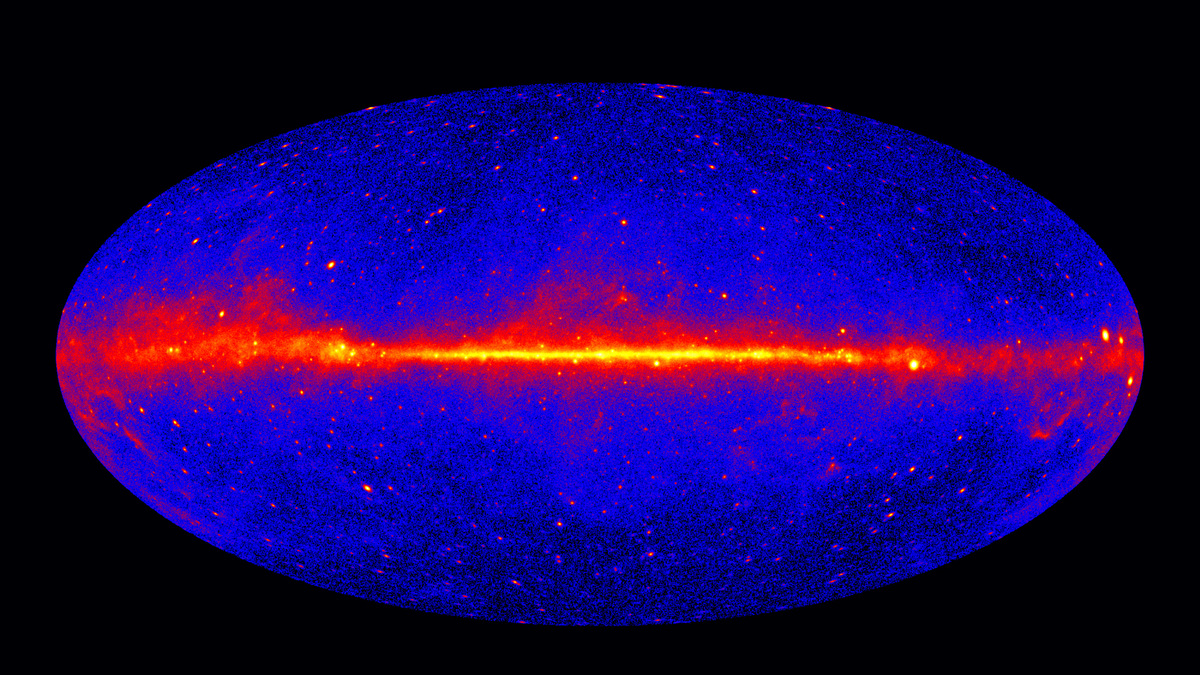
\includegraphics[width=\textwidth]{content/background/figures/Fermi_5_years.jpg}
        \caption{Intensity of $\gamma$-ray $>$ 1 GeV in galactic coordinates (Image credit: NASA/DOE/\textit{Fermi} LAT Collaboration).}
        \label{fig:gamma_galac_plane}
    \end{figure}

    % \item \textbf{Pulsar and Active Galactic Nucleus (AGN)}: 
    % Another source of the brightness in Figure \ref{fig:gamma_galac_plane}
    % is the bright dots with a different solid angle width in the sky.
    % The majority of those spots consists of $\gamma$-ray from 
    % pulsar's periodic emission and AGN or extremely luminous AGN
    % namely "Quasar". The cycle of the lighthouse effects from pulsar 
    % is very robust as in the scale of an atomic clock. Both of them 
    % has a very high magnetic field strength. Emissive photons from 
    % those sources would be very high energy due to the accelation 
    % of a charged particle near magnetic poles or the outer.

    \item \textbf{Pulsars}: 
    Pulsars are rapidly spinning neutron stars as a result of
    the supernova explosion of massive stars.
    They have very strong magnetic fields and can emit bright
    radiation in a beam from their magnetic poles.
    The pulsars' intensity could appear to be a periodic
    emission to observers on Earth due to the pulsars' rotation.
    They are likely the majority of point sources in the Galactic
    plane region detected by \textit{Fermi} LAT.

    \item \textbf{Active Galactic Nuclei (AGNs)}: 
    AGN is the center of the active galaxy.
    The luminosity is much higher than the stars.
    It produces multi-wavelengths
    photon in a different band such as radio,
    microwave, $\gamma$-ray and etc.    
    Then this object could be observed from various instruments.
    
    
    % \textcolor{red}{Write this..}

    \item \textbf{Earth's limb $\gamma$-ray production}:
    The closest $\gamma$-ray source to the LAT is our Earth's atmosphere.
    The Earth's upper atmosphere is extremely bright 
    in $\gamma$-ray band. The Earth shines in high energy
    ($>$100 MeV) $\gamma$ ray due to the collisions of CRs with
    the Earth's upper atmosphere producing secondary particles
    which include $\pi^0$'s that quickly decay into $\gamma$ rays.
    The Earth's $\gamma$-ray emission is the main target source
    for this study.
    % in $\gamma$-ray exposure. The main reason that causes the shining 
    % of Earth's limb does come from the collision of the CR's massive
    % particle such as protons and alphas. The interaction of those high 
    % energy CR massive particles yields many more particles and main 
    % contribution of the $\gamma$-ray dazzling came from the neutral pion
    % decay which is the product of the collision process.

\end{itemize}



%%%%%%%%%%%%%%%%%%%%%%%%%%%%%%%%
%         Fermi-LAT
%%%%%%%%%%%%%%%%%%%%%%%%%%%%%%%%
\section{\textit{Fermi} Large Area Telescope (LAT)}
One of the famous space telescopes that
% do see the sky in the visible wavelength is
observes the sky in $\gamma$-ray wavelength is the
\textit{Fermi} Large Area Telescope (LAT).
Formerly, it was called Gamma-ray Large Area Space Telescope (GLAST).
The LAT is designed to collect high-energy ($\sim$100 MeV to above 300 GeV)
photons data, but it is also able to measure electrons.
% The mission of the satellite is to collect high energy photon data 
% or $\gamma$-ray and it technically could detect the lightweight
% lepton particles namely electron and position.
The orbiting radius is around 550 kilometers
from sea level.
% It is designed for observing the full-sky in 
% $\gamma$-ray region. It also attaches
\textit{Fermi} also carries
the Gamma-ray Burst Monitor (GBM) to study $\gamma$-ray
bursts for seeking exotic events. The telescope was launched
on 11 June 2008 and is still currently taking data in 2021.
% in 11 June 2008 at 16:05 UTC or 21:05 Bangkok time by abroad with 
% Delta II 7920-H rocket.


\subsection{Overview}

\begin{figure}[h!]
    \centering
    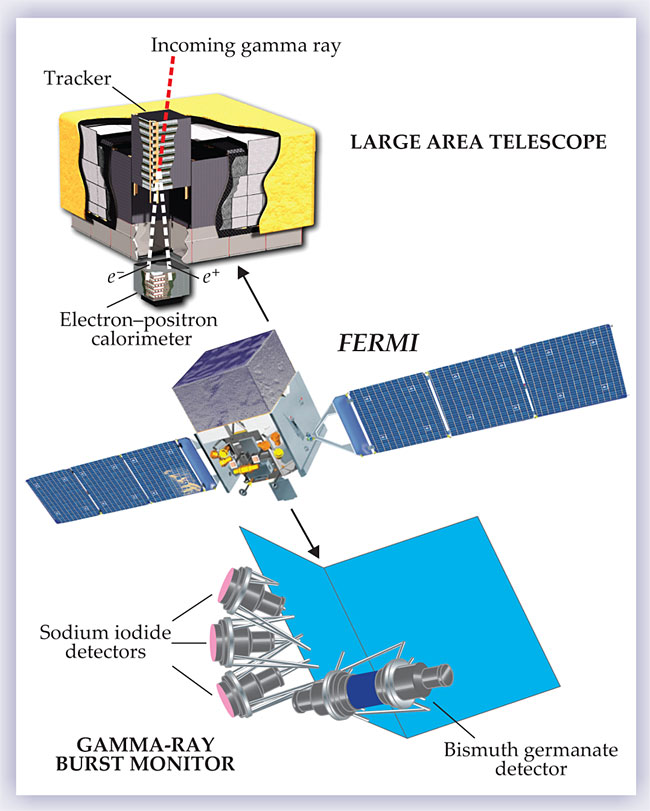
\includegraphics[width=0.6\textwidth]{content/background/figures/fermi_instrument.jpeg}
    \caption{
        Main components of the LAT and the GBM on the \textit{Fermi}
        Space Telescope \citep{fermi_lat_instrument_first_year}}
    \label{fig:fermi_main_components}
\end{figure}

Figure \ref{fig:fermi_main_components} shows
components of \textit{Fermi}.
There are two instruments onboard: the Large Area Telescope (LAT)
and the Gamma-ray Burst Monitor (GBM).
The LAT is the primary instrument that detects $\gamma$ rays
between $\sim$100 MeV to above 300 GeV. The GBM monitors the sky at
a lower energy range of $\sim$8 keV to 40 MeV.
% According to Figure \ref{fig:fermi_main_components},
% each component of the telescope was designed for a purpose since there 
% is no ideal detector module that could detect kind of particles.
% There are two main parts where the first part is the major component 
% called Large Area Telescope (LAT) for detecting the $\gamma$
% -ray and the second part is Gamma-ray Burst Monitor (GBM) for seeking 
% an interesting event in the sky. Both of them do detect 
% the $\gamma$-ray but in the different energy scale. LAT is the main 
% component where it detects the $\gamma$-ray in a few dozen of GeV 
% up to a digit of TeV. For the GBM part, the visible photon energy 
% for them is around 8 keV to 40 MeV.
The GBM consists of two 
sub-components which are sodium iodide detector for low-energy photons
(8 keV to 1 MeV) and bismuth germanate detector for high-energy photons 
(0.2 MeV to 40 MeV).
The GBM monitors transient events and immediately triggers the
LAT to point to the locations of the flares for a certain period
of time before returning to the normal survey mode.
% GBM detectors distribute around 
% the telescope to be a closed circuit camera and looking for a flare 
% of the $\gamma$-ray. The actual purpose of GBM is not a detector 
% for collecting a high quality data but it is attached in the spacecraft 
% to assist the LAT in mainly looking at an interesting event that could 
% produce a huge amount of $\gamma$-rays. The content in this chapter 
% will deep down into more detail of LAT depth and would not provide 
% more detail of GBM.

\subsection{Large Area Telescope (LAT)}


\begin{figure}[h!]
    \centering
    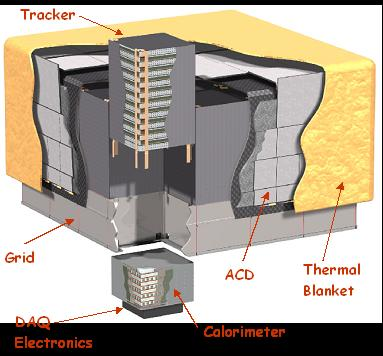
\includegraphics[width=0.6\textwidth]{content/background/figures/LATStructure.jpg}
    \caption{Main components of the LAT (Image taken from https://fermi.gsfc.nasa.gov)}
    \label{fig:fermi_lat_structure}
\end{figure}

Figure \ref{fig:fermi_lat_structure} illustrates main components of the LAT
which are described as follows.
% LAT consists of a tracker (TKR) module for tracing the incoming photon,
% calorimeter (CAL) for measuring the kinetic energy after the particle 
% has been passed through the tracker because a charged particle 
% interact with the CAL and dissipate since it enters the module
% and anti-coincidence Detector (ACD) for rejecting the background 
% signal. The last part is the onboarding data acquisition (DAQ)
% module for investigating the particle's footprint and digitize
% the signal.




\subsubsection{Anti-coincidence Detector (ACD)}
The ACD consists of 89 plastic scintillator tiles covering four
sides and the top of the LAT. Each tile contains two
photomultipliers and wavelength shifting fibers embedded
in the scintillator. The edges of neighboring tiles are
overlapping to reduce the effect of the gaps.
The main objective of the ACD is to reject background
charged particles which create electrical signals when
passing through the scintillator tiles.
The estimated efficiency for charged particle identification
by the ACD is about 0.9997.
% \textcolor{red}{rewrite backsplash}

% (อ่านเรื่อง backsplash ไม่รู้เรื่อง ถ้าอยากเขียนจริงๆ เขียนมาใหม่)

% The main objective of ACD is to support the charged-particle background rejection of the CRs. It is cover the tracker over the LAT field of 
% view (FoV) for 4 sides and the top part of the LAT. It consists of 
% 89 plastic scintillator tiles with 5 $\times$ 5 array on top and 
% 4 sides of 16 tiles. Each tile component contains two photomultiplier 
% and wanelength shifting fibers embedded in the scintillator. The tile 
% is overlapping another one in one dimension to reduce the effect of 
% the gaps between them. To be more precise, there are two sets 
% of four called scintillator ribbons for covering the top-down side 
% and a pair around their center. The ACD is required to has 0.9997 efficientcy 
% for detecting an incoming charged particle of FoV of the LAT. However,
% the $\gamma$-ray induces the shower that the calorimeter will absorb but 
% there is a scenario called the "backsplash effect" where the secondary 
% particles in keV range from the electromagnetic shower could interact 
% with the incoming photon and Compton scattering in ACD. Then it could 
% create a veto signal from the recoil electron. To solve this issue,
% the ACD with their neighborhood would take the incident candidate photon 
% into account and could dramatically reduce the effect of the back splashing.




\subsubsection{Tracker (TKR)}

\begin{figure}[h!]
    \centering
    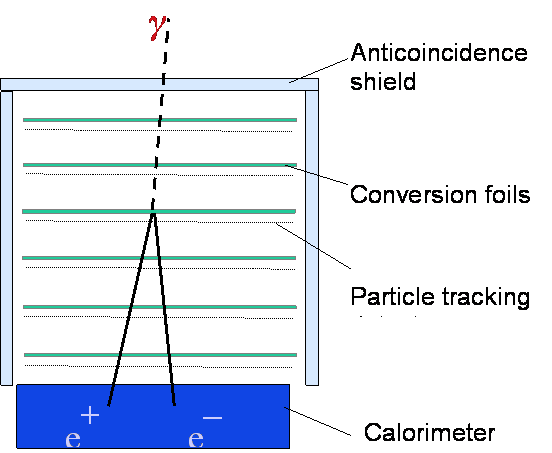
\includegraphics[width=0.6\textwidth]{content/background/figures/LAT_layers.png}
    \caption{
        Schematic of $\gamma$-ray detection of the LAT
        (Image taken from https://fermi.gsfc.nasa.gov)
    }
    \label{fig:fermi_lat_layers}
\end{figure}


The TKR system consists of 16 planes of particle tracking detectors
made from silicon strips which are interleaved with tungsten
conversion foils as shown in Figure \ref{fig:fermi_lat_layers}.
An incident
$\gamma$ ray has high probability to interact with the conversion
foil and is converted into an $e^+e^-$ pair. 
% Higher energy photon or $\gamma$-ray talk to the LAT by converting the
% kinetic energy into a pair of lightweight leptons or e$^{+}$e$^{-}$ pair.
% The converter-tracker has 16 planes of a large atomic number for 
% making the incident $\gamma$-ray convert into a pair of e$^{+}$e$^{-}$
% as demonstrated in Figure \ref{fig:fermi_lat_layers}. After that, 
% a pair of leptons would leave a footprint as an electromagnetic induction 
% in particle tracker where it sensitive for the moving charged particle.

\begin{figure}[h!]
    \centering
    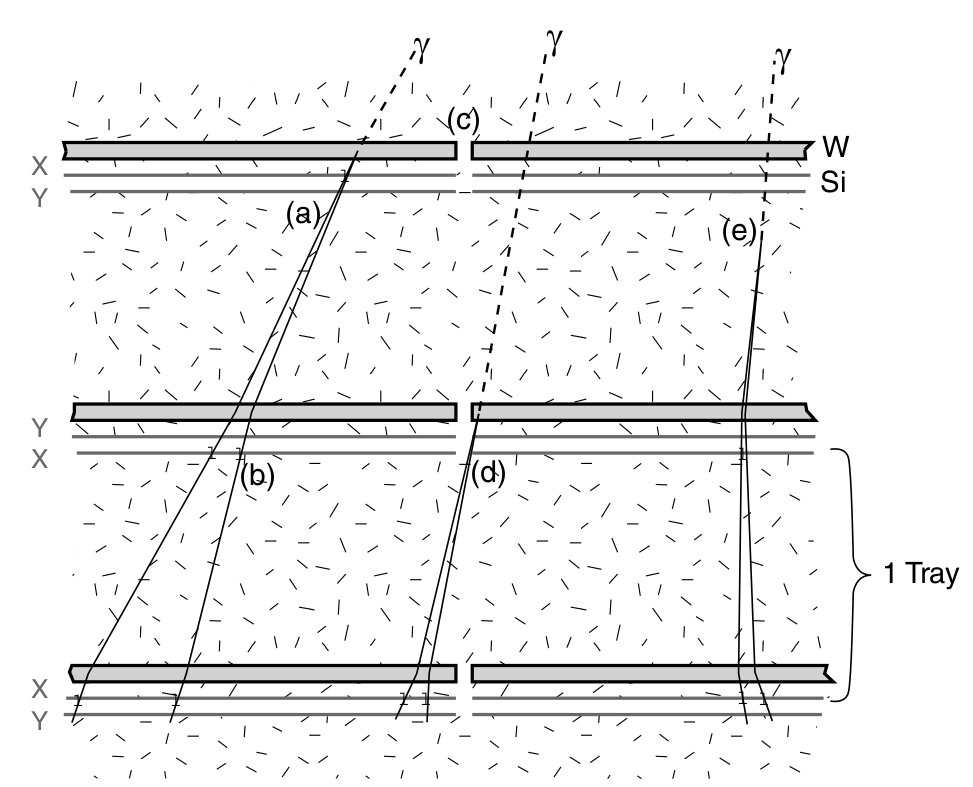
\includegraphics[width=0.6\textwidth]{content/background/figures/fermi_tracker.png}
    \caption{
        LAT's particle tracker.
        (a) The ideal case where the conversion happens in an early
        layer and leaves a footprint along with multiple layers (b).
        (c) The photon skips the first layer and be converted in another layer
        with a missed hit in 1st and 2nd of Si trackers (d).
        (e) Conversion occurs in structural materials and is traced 
        by the following Si trackers.
        \citep{FermiLAT}
    }
    \label{fig:fermi_tracker}
\end{figure}

As the $e^+e^-$ pair travel through the silicon strip trackers,
they leave their traces on the position sensing detectors,
allowing us to reconstruct the direction of the original photon.
The narrow gaps between layers of silicon trackers improve the
angular resolution of the LAT compared to previous instruments.
In Figure \ref{fig:fermi_tracker},
case (a) is the typical situation in which photon
is pair-produced by the conversion layer and clean $e^+e^-$
footprints are recorded. Nevertheless, there are some cases,
such as (d) in which the $e^+e-$ paths pass through the gap
between towers or (e) in which the photon is pair-converted
outside of the conversion foil. Having multiple layers of
trackers helps the reconstruction of these special cases.

% The particle tracking is made from silicon strips. Tracking information 
% would leave the track in a 2-D plane of particle tracking. In order to
% traceback and gaining data as the 3-D moving direction, 16 particle 
% tracker has to be taken into account for constructing the electron 
% or positron path.
% Despite one layer of particle tracking could obtain 
% the information about incoming leptons for x-y plane only, but technical 
% design of LAT does put 2 layers of the silicon-based tracker with a very 
% narrow gap between them. This kind of design could make the LAT performing 
% measurement precision in the angular resolution better than a single 
% layer of a wide gap which affects the point-spread function (PSF)
% of the probability distribution from reconstruction direction.
% According to Figure \ref{fig:fermi_tracker}, the top and the bottom of
% silicon trackers and the heavy-nuclei conversion layer called "Tray".
% Case (a) and (b) in the figure is the ideal case where the $\gamma$-ray
% hit the conversion layer and multiple footprints are recorded.
% Nevertheless, there is an edge case as in (d) and (e) where the $\gamma$-ray
% has a probability to skip an early layer and choose to covert in the 
% secondary conversion layer and will be detected in the upcoming 
% tracking layer. The major benefit of deploying multiple conversion 
% layers are quite obvious for a better event gathering.


\subsubsection{Calorimeter (CAL)}

When the $e^+e^-$ pair enters the CAL, they radiate their energy
in the CsI crystal scintillators, producing electronic readout
which is proportional to the energy loss of $e^+e^-$ inside the CAL.
According to the radiation lengths of $e^+$ and $e^-$,
the CAL is optimized to contain the $e^+e^-$ showers with
energy from ~0.1 to a few hundred GeV. Thus, TeV photons
could have large uncertainties in their energy reconstruction
by the LAT.
% Unlike particle tracker that talks to a charged particle by utilizing
% the EM induction without (or barely) disturbing the particle state,
% the calorimeter is a starving component. It consumes a lepton and produce 
% electronic readout of the energy from the radiation of the lepton in the
% crystal scintillator. The size of this part is mainly considered 
% from the radiation lengths of the electron and position particles becasue it has to record the shower that happens during the decaying process.
% However, the radiation length highly depends on the kinetic energy 
% of the particle. The LAT itself has been designed for detecting photon 
% energy range between MeV to a few hundred GeV. Hence, the exposure of 
% photon energy beyond TeV is probably not promising in this case.


\begin{figure}[h!]
    \centering
    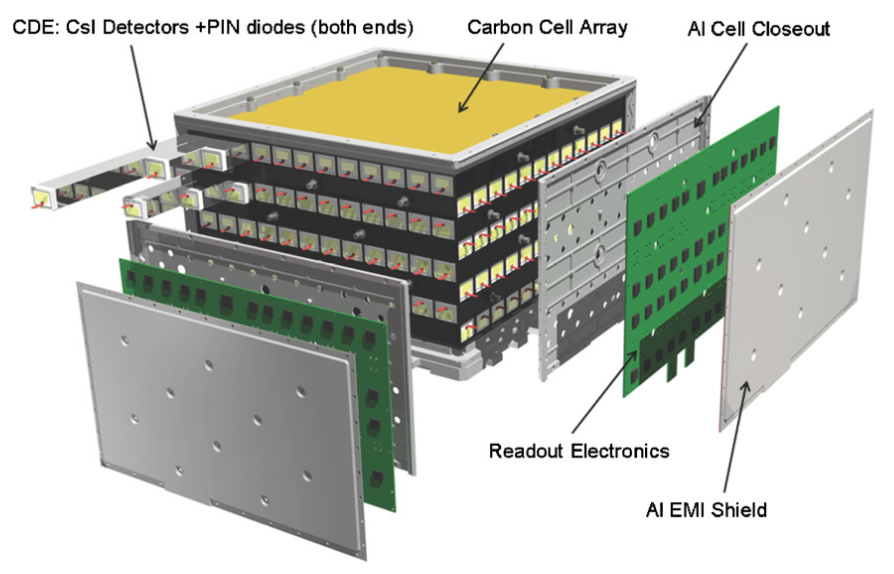
\includegraphics[width=0.8\textwidth]{content/background/figures/fermi_calorimeter.png}
    \caption{LAT's calorimeter \citep{FermiLAT}}
    \label{fig:fermi_calorimeter}
\end{figure}

The overview apparatus structure is illustrated in Figure \ref{fig:fermi_calorimeter}.
Each calorimeter module consists of 96 CsI(Tl) scintillator
crystals with the size of
2.7 cm x 2.0 cm x 32.6 cm and PIN photodiodes at both ends which connect 
to the readout electronic components translating the amount of light 
sparkled in the crystal to digitized signals. Each horizontal 
layer is combined from 12 crystal components and stack 8 times by 
rotating them 90\textdegree each for boosting the angular resolution 
for the sparking lights. A carbon cell was build for supporting 
the structure of low mass particle tracker due to the properties of 
high stiffness, thermal conductivity and thermal stability.
An electron, position, or $\gamma$-ray will deposit the energy in the
calorimeter as the scintillated lights via electromagnetic interactions.
The segmented
crystal allow LAT to trace the showers of particles for spatial imaging.
% crystal also allows LAT to trace the shower
% as the spatial imaging.




\subsubsection{Data Acquisition System (DAQ)}

% To acquire an interesting event, event selection could not be done on software on the ground level from the whole raw signal of subsystems because of the limitation of the hardware in the current edge. To collect an event, 
% raw data will be selected from the filtering algorithm on board.
% The hierarchical structure of data acquisition system (DAQ) was invented 
% for seeking a transient event as shown in Figure \ref{fig:fermi_daq}.

\begin{figure}[h!]
    \centering
    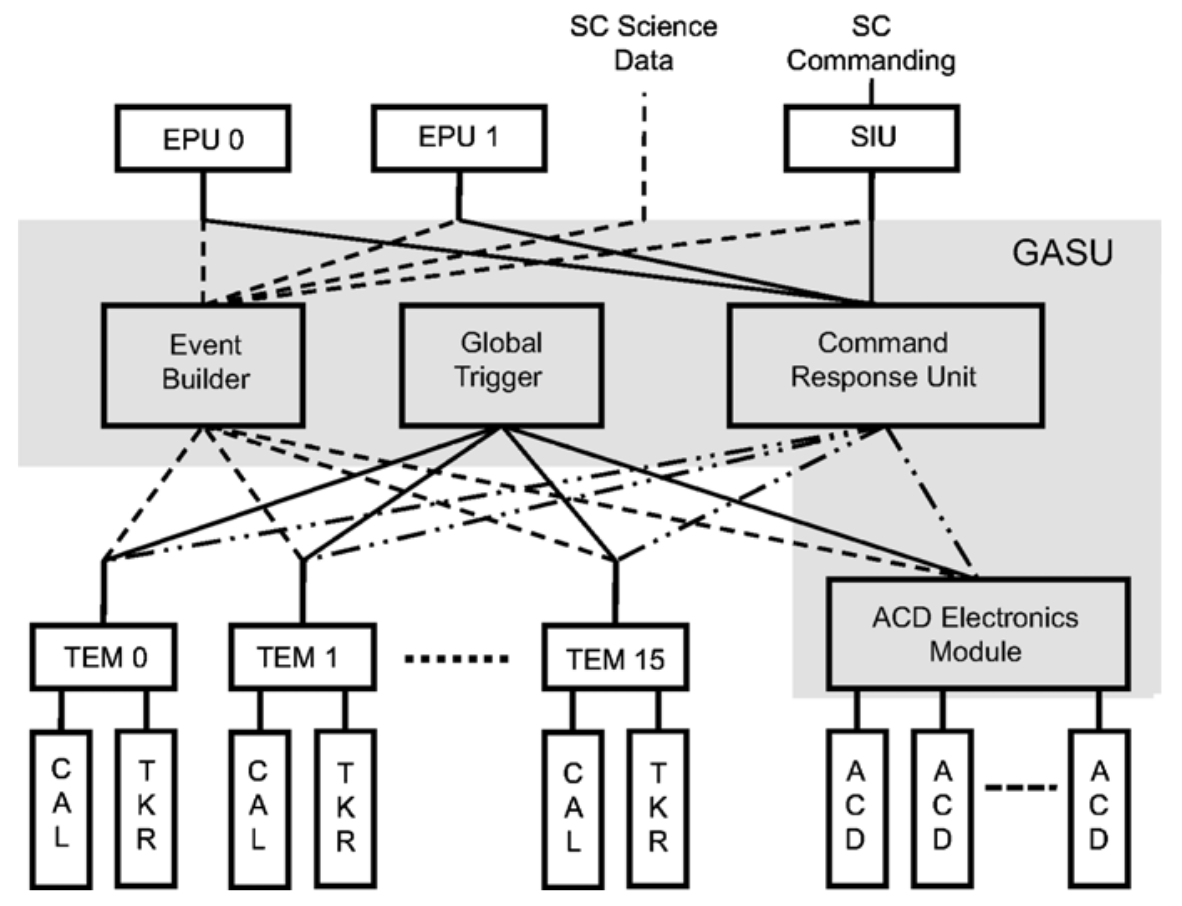
\includegraphics[width=0.6\textwidth]{content/background/figures/fermi_daq.png}
    \caption{Flow chart of LAT's data acquisition system (DAQ) (Image taken from \citealt{FermiLAT})}
    \label{fig:fermi_daq}
\end{figure}

The DAQ system is designed to reduce the amount of raw data
transmitted to the ground through the limited bandwidth. 
The lowest-level components are tower electronic modules
(TEMs) to serve as the interface for the the TKR and CAL.
All TEMs create event 
buffering and communicate with the Event Builder Module (EBM) which is a
component of Global-trigger/ACD-module/Signal Distribution Unit (GASU).
Command Response Unit (CRU) is built to communicate the
software execution in the DAQ system. Lastly, the Event Processing Unit (EPU)
processes a selected event from TEM and ACD Electronics Module (AEM).
Filtering an event could reduce the data transmission rate from 
a few kHz to around 400 Hz to the ground level.


\subsection{Event reconstruction}

Before launch, the event reconstruction algorithm for photons
was based entirely on the Monte Carlo (MC) simulations by
modeling the photon and background signals in the ACD, TKR,
and CAL systems in realistic in-orbit environment.
The data processed by this pre-launch event reconstruction
algorithm is called ``Pass 6'' version.

% In an early day, the reconstruction algorithm for tracing a photon 
% is Monte Carlo (MC) simulation. Modeling the incident $\gamma$-rays 
% and the background has been simulated in the orbiting-like environment 
% before it launches. Meaning that background rejection property already 
% embedded in the LAT since the developing process. The simulation 
% could be use for the detector calibration since the simulation software 
% provide an interactive physical process.

% The main logic of the reconstruction is to start by tracking the footprint 
% in the tracker and expect the output in the calorimeter cube as physical process 
% would yield. After that, the event classification mainly consider from 
% the ACD part to classify an event type.

The raw onboard data are called ``level 0''. After transmitted 
to the ground and processed, the data become ``level 1''.
After a few years after launch, the LAT collaboration has
improved the event reconstruction algorithm and released
the ``Pass 7'' version based on the actual in-flight data.
% The result from processed data on the fly is level 0 and it will pass 
% down to Earth and reconstructing the photon data called level 1.
% The more LAT orbiting around the Earth's, the more understanding of the 
% LAT environment and it brings the software improvement for the reconstruction
% algorithm to exploit the technique of pattern recognition.
% The first official release is LAT data is Pass 6 and Pass 7 after has been 
% released with the same level 0 data but the reconstructed event is 
% more efficient than the older one by software level.
The newest version 
and likely to be the final version is Pass 8.
In each version, photons are organized into different classes
(e.g., TRANSIENT, SOURCE, ULTRACLEAN, ULTRACLEANVETO)
based on the level of background contamination.
The TRANSIENT class has the loosest selection which allows us
to obtain better statistics for the observations of faint
transient sources but with a trade-off for the highest
probability of background contamination.
The SOURCE class is optimized for typical source
analyses of the LAT, while the ULTRACLEANVETO is the
cleanest class with low background contamination but
also with the lowest statistics.
% Not only the reconstruction
% algorithm that has been divided but the event class is also an 
% crucial concept. As mentioned earlier, the photon is classified into 
% a specific class. There is no free lunch to think that the detector see 
% the particle as a binary classification. It will mix with a likelihood or probability to distinguish the specific kind of interesting event.
% That is the main reason why \textit{Fermi}-LAT team split the event 
% into multiple classes which mainly are TRANSIENT, SOURCE, ULTRACLEAN and 
% ULTRACLEANVETO.

% Lesser photon candidates have been selected in the ULTRACLEANVETO. Then there is no certain right or wrong for
% picking the class from the researcher's point of view. The main criteria would be the objectives of the analysis. If the analyzer wants to collect as much events as possible and could accept some noisy event, then SOURCE or 
% TRANSIENT class is suitable for the analysis and vice versa.


\subsection{LAT performance and characteristics}

\begin{figure}[h!]
    \centering
    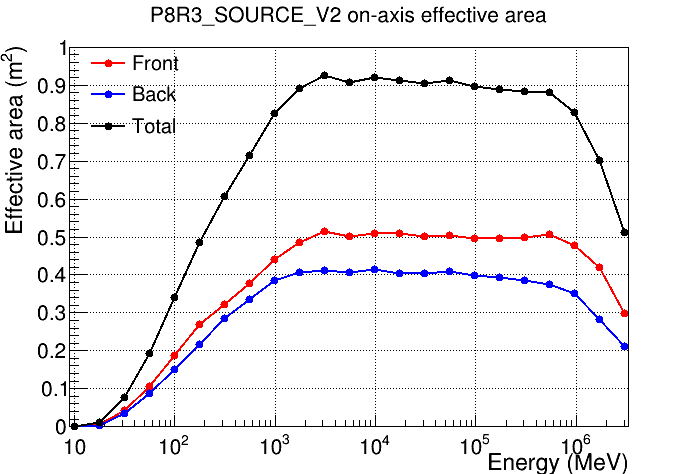
\includegraphics[width=0.7\textwidth]{content/background/figures/eff_energy.png}
    \caption{
        LAT's effective area as a function of energy
        for normally incidence photons \citep{lat_p8_performance}.
        Front means the effective area of an event that photon hits
        the conversion layer at the top and decays into
        a pair of electron-position.
        Back represents the effective area of the event that photons
        pass through the top part and be converted to the bottom of 
        the TKR module. The total effective area (black)
        is the combination of front and back.
    }
    \label{fig:eff_energy}
\end{figure}

\textit{Fermi} LAT's physical cross-section area is 1.8 x 1.8 m$^2$.
However, its effective area for particle detection varies as a
function of energy and incidence angle. Figure \ref{fig:eff_energy}
shows the LAT's Pass 8 SOURCE effective
area for photons arriving
perpendicular to the cross section of the LAT as a function
of energy, indicating low detection efficiency below $\sim$100 MeV
and above $\sim$1 TeV.
The effective area from front part is higher than the back due to 
the conversion event that happens in the front 
leaves more footprint in silicon strip of TKR more than the back.

% \textit{Fermi}-LAT has been designed for detecting $\gamma$-ray in the 
% space which means that the range of energy that it could see precisely 
% will be starting at MeV up to TeV. The effective area in square-meters
% is defined from the front and the back of the LAT's tracking layer 
% by considering the upper part as a front and the bottom part belowing 
% a certain layer as the back part. Since both front and back part components are made by the same materials and exactly the same design. 
% Then total effective area could be sum into a single value. 
% Figure \ref{fig:eff_energy} visualize the effectiveness of LAT 
% along with a given energy range. According to the plot, LAT performs 
% a measurement well from GeV up to TeV scale.

\begin{figure}[h!]
    \centering
    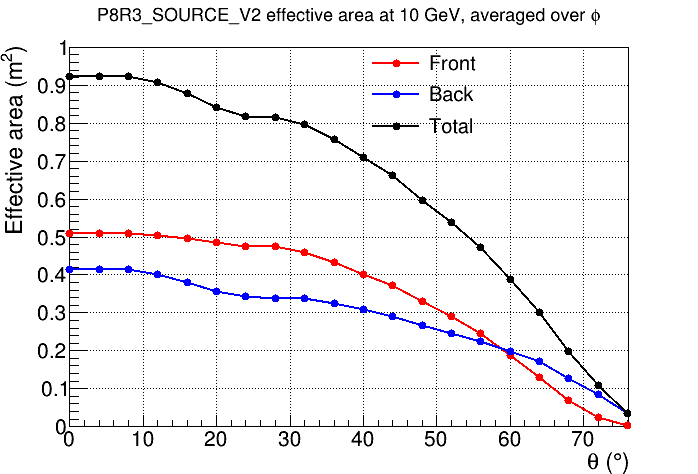
\includegraphics[width=0.7\textwidth]{content/background/figures/eff_theta.png}
    \caption{
        Effective area versus incidence angle \citep{lat_p8_performance}
    }
    \label{fig:eff_theta}
\end{figure}

Another crucial variable relating to the LAT effectiveness
is the incidence angle ($\theta_\text{LAT}$).
An event with small $\theta_{\rm LAT}$ would pass through many
tracking layers, yielding better detection efficiency.
% It highly affects the number of tracking layers.
% The higher probability of passing more tracking layers
% would yield a better LAT's performance.
Figure \ref{fig:eff_theta} shows
the relation between the effective area and $\theta_{\rm LAT}$.
% relation of effective area versus 
% incidence angle.

% 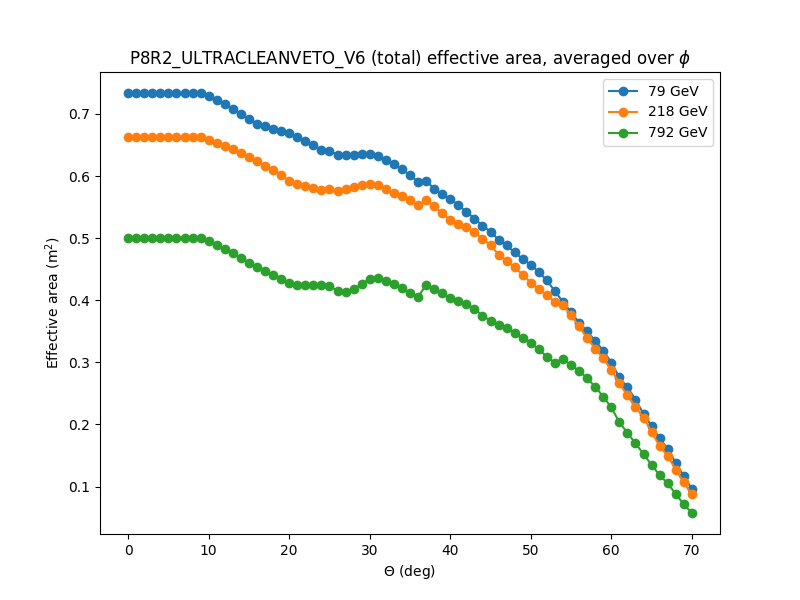
\includegraphics[width=0.8\textwidth]{content/background/figures/custom_eff_theta.png}
%     \caption{Effective area versus incidence angle (sampled from 3 energies)}

% angle dependency 

\begin{figure}[h!]
    \centering
    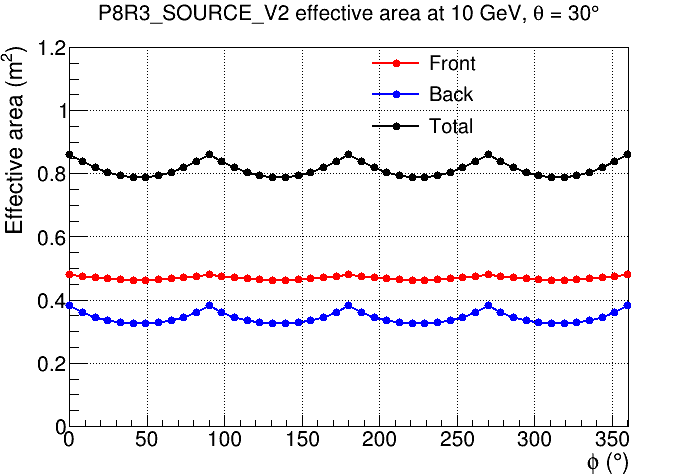
\includegraphics[width=0.7\textwidth]{content/background/figures/eff_phi.png}
    \caption{
        Effective area versus $\phi_\text{LAT}$ \citep{lat_p8_performance}
    }
    \label{fig:eff_phi}
\end{figure}


Since the structure of the LAT is cube-like, the effective area,
therefore, depends on the azimuthal angle
($\phi_\text{LAT}$) of the photon. Figure \ref{fig:eff_phi} illustrates
the asymmetry of the LAT's effective area as a function of
$\phi_{\rm LAT}$, showing four peaks corresponding to corners
of the LAT.
% Imagine the LAT structure as a cube-like detector. Surely, the LAT 
% boresight is a square where an azimuthal angle ($\phi_\text{LAT}$) of the incoming 
% photon would affect a larger area that the photon could interact 
% as demonstrates in Figure \ref{fig:eff_theta}. The reason why there 
% is a peak for any cycle of $\pi/2$ radian or 90\textdegree is 
% the edge of the LAT would have more area to interact than the 
% lateral. Another evidence for the explanation is the front effective 
% area has fewer effects since the propagation length is narrow than 
% the back.

% \begin{figure}[h!]
%     \centering
%     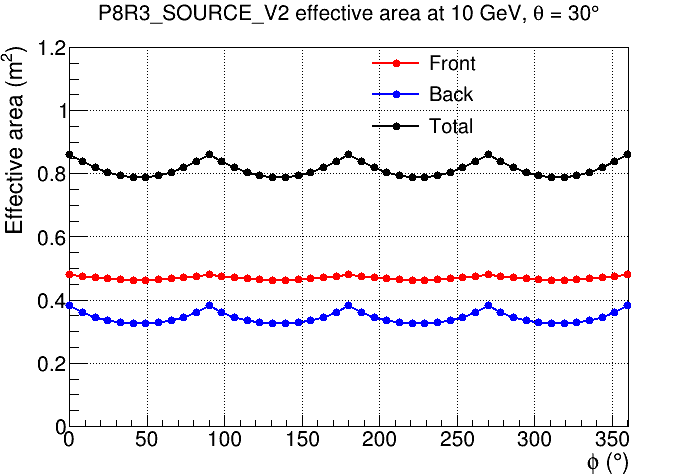
\includegraphics[width=0.7\textwidth]{content/background/figures/eff_phi.png}
%     \caption{
%         LAT's effective area versus azimuthal angle for
%         a 10 GeV photon with the incidence angle
%         of 30$^\circ$ \citep{lat_p8_performance}.
%         % Effective area versus azimuthal angle \citep{lat_p8_performance}
%     }
%     \label{fig:eff_phi}
% \end{figure}

% event class
% \newpage

\begin{figure}[h!]
    \centering
    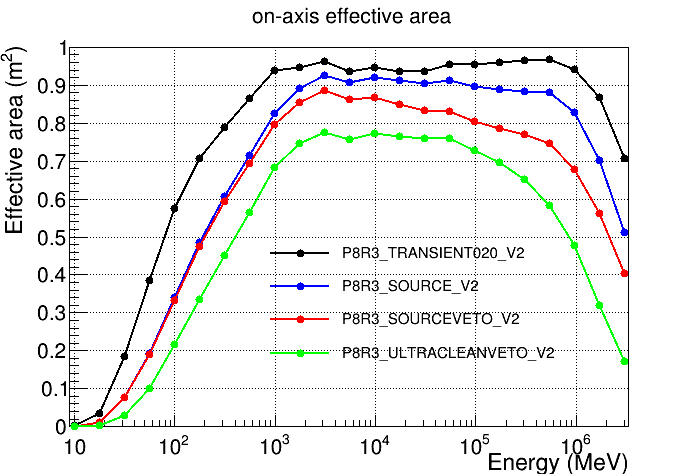
\includegraphics[width=0.7\textwidth]{content/background/figures/eff_event_class.png}
    \caption{Effective area along with the energy of each event class \citep{lat_p8_performance}}
    \label{fig:eff_event_class}
\end{figure}


The event class also has a crucial role when considering the effectiveness of the reconstructed event.
The cleanest class namely ``ULTRACLEANVETO'' would have the smallest
effective area. On the other hand, the TRANSIENT class would yield 
the largest effective area as illustrated in Figure \ref{fig:eff_event_class}.
Please see Appendix \ref{appendix:cleanveto_eff_area} for the illustration
of the effective area from class ``ULTRACLEANVETO'' that has been selected 
in this work.